% Copyright (C) 2005-2015 Airbus - EDF - IMACS - Phimeca
% Permission is granted to copy, distribute and/or modify this document
% under the terms of the GNU Free Documentation License, Version 1.2
% or any later version published by the Free Software Foundation;
% with no Invariant Sections, no Front-Cover Texts, and no Back-Cover
% Texts.  A copy of the license is included in the section entitled "GNU
% Free Documentation License".
\renewcommand{\filename}{docUC_InputWithData_CopulaKendallPlotTest.tex}
\renewcommand{\filetitle}{UC : Copula validation through the Kendall Plot Test}

% \HeaderNNIILevel
% \HeaderIILevel
\HeaderIIILevel


\label{copula_validation}


\index{Copula!Model Validation}
\index{Fitting Test!Kendall-plot}



The objective of this Use Case is to exhibit the different uses of the Kendall Plot to :
\begin{itemize}
\item test a specific model of bivariate copula with respect to a sample,
\item test whether two bivariate samples share the same copula model.
\end{itemize}


Details on the Kendall Plot Test may be found in the Reference Guide (\extref{ReferenceGuide}{see files Reference Guide - Step B -- Graphical googness-of-fit tests : QQ-plot, Kendall Plot and henry line.}{stepB}).\\


This Use Case performs the following analysis :

In the example, we suppose we have a sample of dimension 2. The objective is to estimate the dependence structure of the sample. The analysis  has the following steps :
\begin{enumerate}
\item  we suppose we have a sample of dimension 2 $sample1$ and a given model of copula \textit{copula} , whatever the way it has been determined (parametric estimation or non parametric one). We want to validate this copula model with the Kendall Plot test, thanks to the method \emph{VisualTest.DrawKendallPlot(sample1, copula)};
\item we suppose we have two samples of dimension 2 $sample1$ and $sample2$. We wonder whether this two samples have the same copula model, whithout specifying it, using the Kendall Plot test, thanks to the method \emph{VisualTest.DrawKendallPlot(sample1, sample2)}.
\end{enumerate}

In OpenTURNS, the mean of the statistics $W_i$ is evaluated with the Monte Carlo sampling method from $n$ simulations. By default, $n=100$. It is possible to change this value thanks to the \textit{ResourceMap} class (see the python script).


\requirements{
  \begin{description}
  \item[$\bullet$] two 2D numerical sample (data) : {\itshape sample1, sample2}
  \item[type:]  NumericalSample
  \end{description}
}
             {
               \begin{description}
               \item[$\bullet$] a bivariate copula : {\itshape copula}
               \item[type:] CopulaImplementation
               \end{description}
             }

             \textspace\\
             Python script for this UseCase :

             \inputscript{script_docUC_InputWithData_CopulaKendallPlotTest}

             \textspace\\

             In Figures  \ref{GoodCop} to \ref{DifCop}, the data 1 and data 2  have been generated from a $Frank(1.5)$ copula, and data 3 from a $Gumbel(4.5)$ copula.\\
             Figures \ref{GoodCop} and \ref{BadCop} respectively validates and invalidates the \textit{Frank} copula model to data 1 and data 2.\\
             Figures \ref{SameCop} and  \ref{DifCop} respectively validates that data 1 and data 2 share the same copula, and shows that data 1 and data 3 don't share the same copula.\\


             \begin{figure}[H]
               \begin{minipage}{10cm}
                 \begin{center}
                   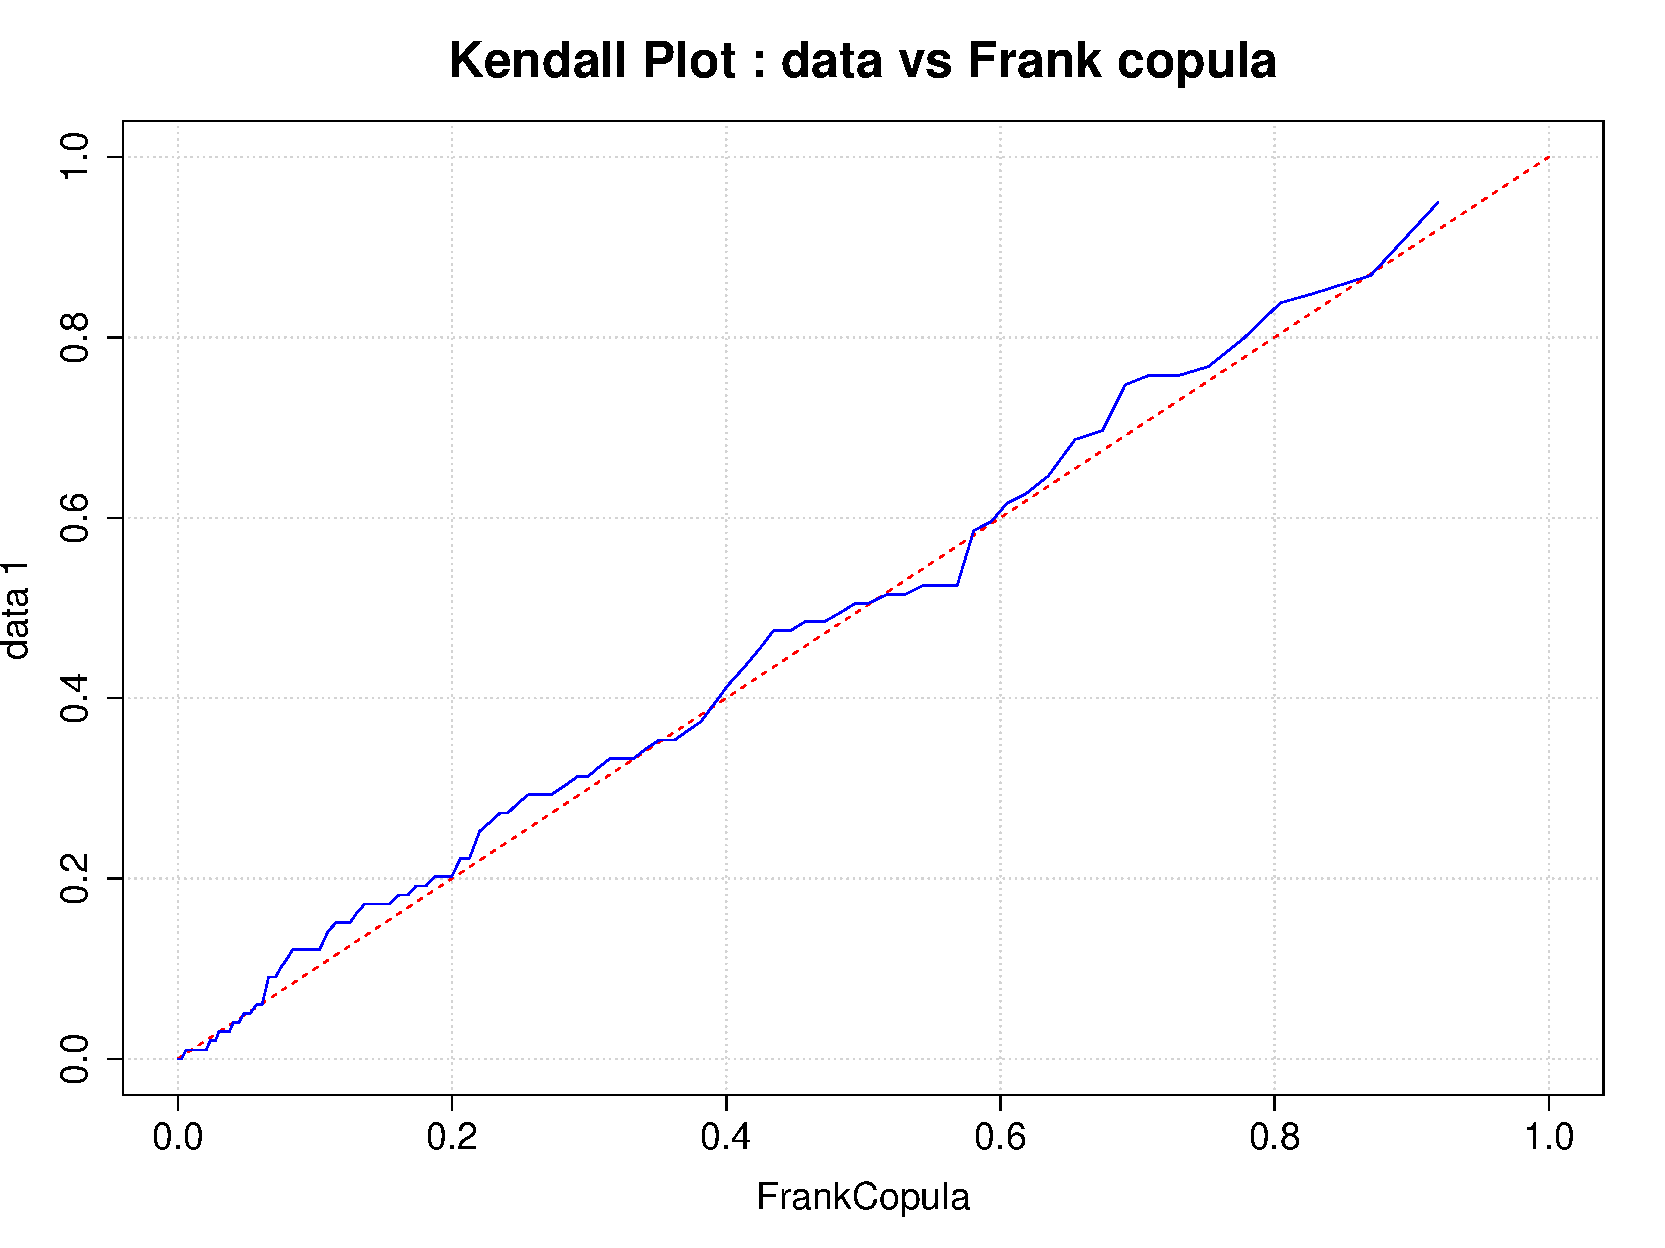
\includegraphics[width=10cm]{Figures/KendallPlotCopula.pdf}
                 \end{center}
                 \caption{The Kendall Plot test validates the use of the Frank copula model for the data 1.}
                 \label{GoodCop}
               \end{minipage}
               \hfill
               \begin{minipage}{10cm}
                 \begin{center}
                   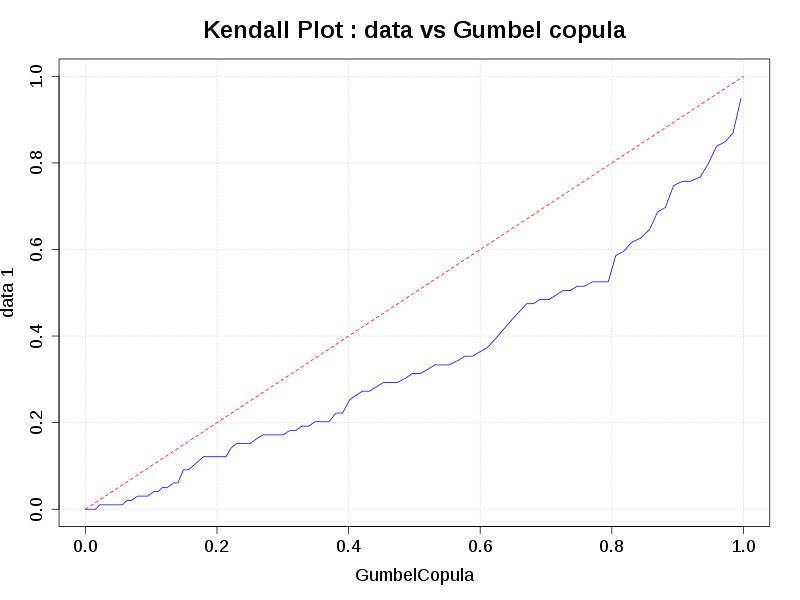
\includegraphics[width=10cm]{Figures/KendallPlotCopulaBad.png}
                 \end{center}
                 \caption{The Kendall Plot test invalidates the use of the Frank copula model for the data 1.}
                 \label{BadCop}
               \end{minipage}
             \end{figure}


             \begin{figure}[H]
               \begin{minipage}{10cm}
                 \begin{center}
                   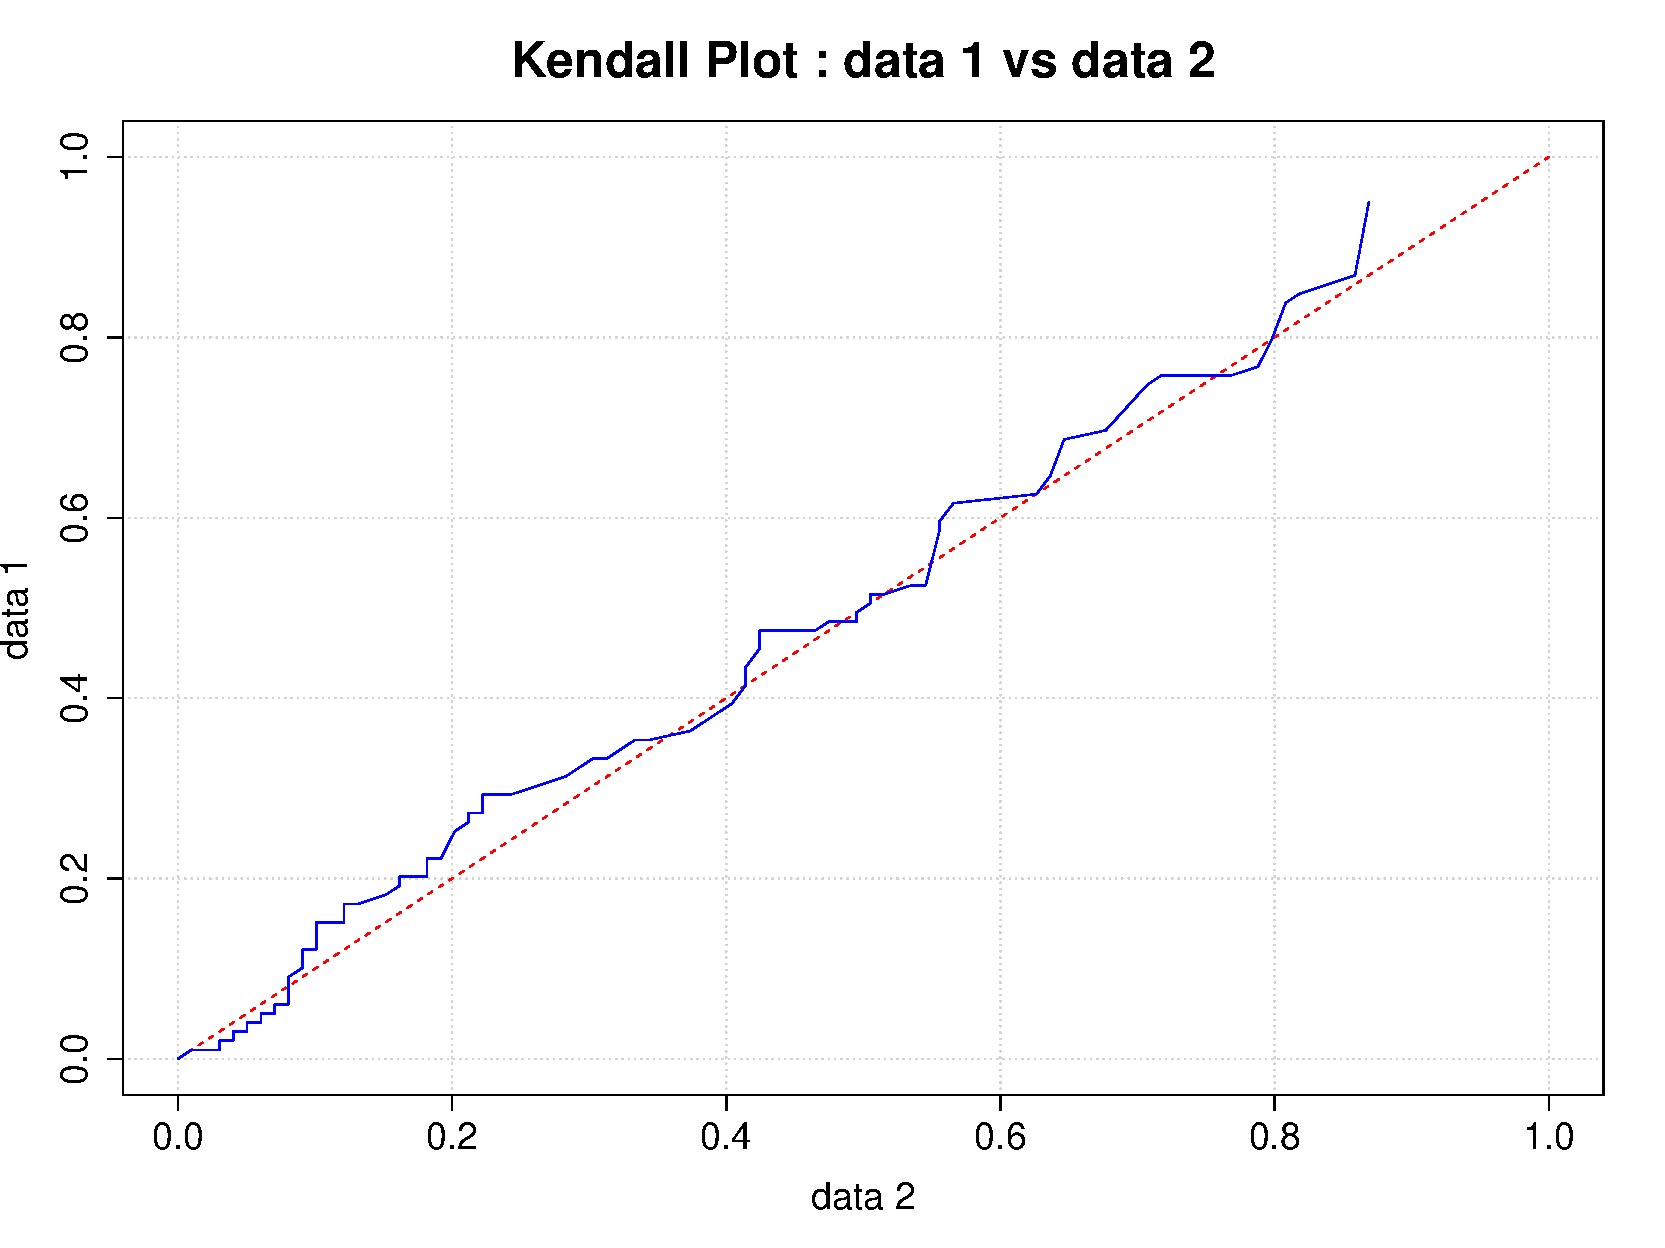
\includegraphics[width=10cm]{Figures/KendallPlotSample.pdf}
                 \end{center}
                 \caption{The Kendall Plot test validates that data 1 and data 2 have the same copula model}.
                 \label{SameCop}
               \end{minipage}
               \hfill
               \begin{minipage}{10cm}
                 \begin{center}
                   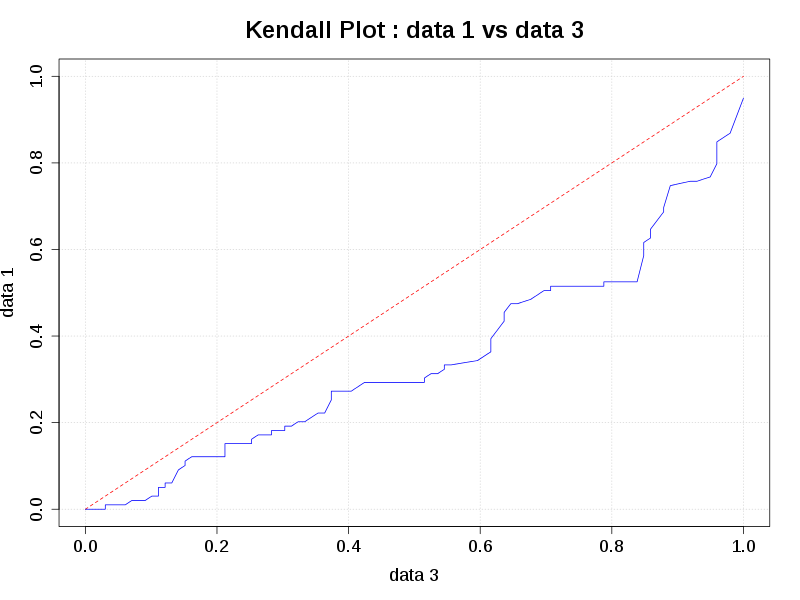
\includegraphics[width=10cm]{Figures/KendallPlotSampleBad.png}
                 \end{center}
                 \caption{The Kendall Plot test invalidates that data 1 and data 3 have the same copula model}.
                 \label{DifCop}
               \end{minipage}
             \end{figure}
